\documentclass[conference,a4paper]{IEEEtran}

\usepackage{amsmath}
\usepackage{array}
\usepackage{cite}
\usepackage{graphicx}
\usepackage{url}

\newcolumntype{P}[1]{>{\raggedright\arraybackslash}p{#1}}

\title{A Sparse-Sensing Spatial Digital Twin for Learning Environmental Impacts of Non-Networked Appliances in a Single Room}

\author{
\IEEEauthorblockN{Yun-You Lin}
\IEEEauthorblockA{
Department of Computer Science and Information Engineering\\
National Changhua University of Education\\
Changhua, Taiwan\\
yunitrish0419@gmail.com}
\and
\IEEEauthorblockN{Chang-Pei Yi}
\IEEEauthorblockA{
Department of Computer Science and Information Engineering\\
National Changhua University of Education\\
Changhua, Taiwan}
\and
\IEEEauthorblockN{Hui-Yu Shen}
\IEEEauthorblockA{
Department of Electrical Engineering\\
Chienkuo Technology University\\
Changhua, Taiwan}
}

\begin{document}
\maketitle

\begin{abstract}
Practical room-scale digital twins must often operate with sparse sensors and non-networked appliances that expose no telemetry. This paper presents a single-room spatial digital twin that estimates temperature, humidity, and illuminance fields from eight corner sensors while modeling conventional air conditioners, manual windows, and ordinary lights. The proposed design combines an appliance-aware bulk-plus-local field model, sparse calibration, appliance-impact learning, and an optional hybrid residual neural layer. Across eight leave-one-scenario-out folds, average field MAE is 0.1723/0.4633/54.9052 for IDW, 0.0474/0.1765/2.0269 for the base estimator, 0.2091/0.2241/48.1422 for a standalone pure RNN without physics estimates, and 0.0017/0.0059/0.1407 for the hybrid; the pure RNN is lowest in 0 of 24 fold-factor comparisons. On a preliminary seven-day bedroom dataset, calibration reduces held-out pillow-point MAE from 0.8967/4.1286/309.0142 to 0.1676/0.3939/16.6450, with positive date-block bootstrap intervals and date-deletion reductions. The evaluation separates controlled full-field evidence, public task-aligned comparisons, and real sparse-calibration checks, supporting complementary roles for physical structure, calibration, and residual learning.
\end{abstract}

\begin{IEEEkeywords}
spatial digital twin, sparse sensing, indoor environment modeling, non-networked appliances, reduced-order model, sensor calibration
\end{IEEEkeywords}

\section{Introduction}
Smart homes and smart buildings require indoor environmental awareness for comfort assessment, energy management, and device control. A practical system should estimate conditions at relevant regions such as a room center, window-side zone, or bed location, not only at installed sensors. This is difficult because dense sensing is intrusive, while ordinary rooms also contain conventional appliances that do not report state, power, or operating parameters.

This work targets a common but under-instrumented digital-twin setting: the room contains influential physical assets, but those assets are not necessarily connected to a building management system. The twin must therefore infer appliance state effects from sparse environmental observations, support what-if queries, and keep its claim boundary clear. Pure interpolation ignores appliance geometry and directionality, while a purely local field model misses whole-room settling after air-conditioner activation. We therefore use a reduced-order appliance-aware model as the primary estimator and evaluate, rather than deploy, an end-to-end pure RNN field baseline alongside structured residual correction.

The contributions are: (i) a three-factor room digital twin with bulk-plus-local appliance influence functions, photometric lamp falloff, and one-bounce diffuse illuminance reflection; (ii) a sparse-sensor calibration pipeline combining active-device power fitting, trilinear residual correction, and before/after impact learning; (iii) a hybrid residual pathway that preserves the reduced-order estimator while refining systematic error; and (iv) an implementation and validation hierarchy covering synthetic full-field scenarios, ablations, leave-one-scenario-out residual learning, window-condition cases, public task-aligned datasets, and preliminary real-bedroom snapshots. Figure~\ref{fig:architecture} summarizes the argument chain from the research gap through methods and evidence to the claim boundary; it also keeps the MCP-compatible interface secondary to the modeling contribution and marks intervention-based recommendation validation as future work.

\begin{figure*}[t]
\centering
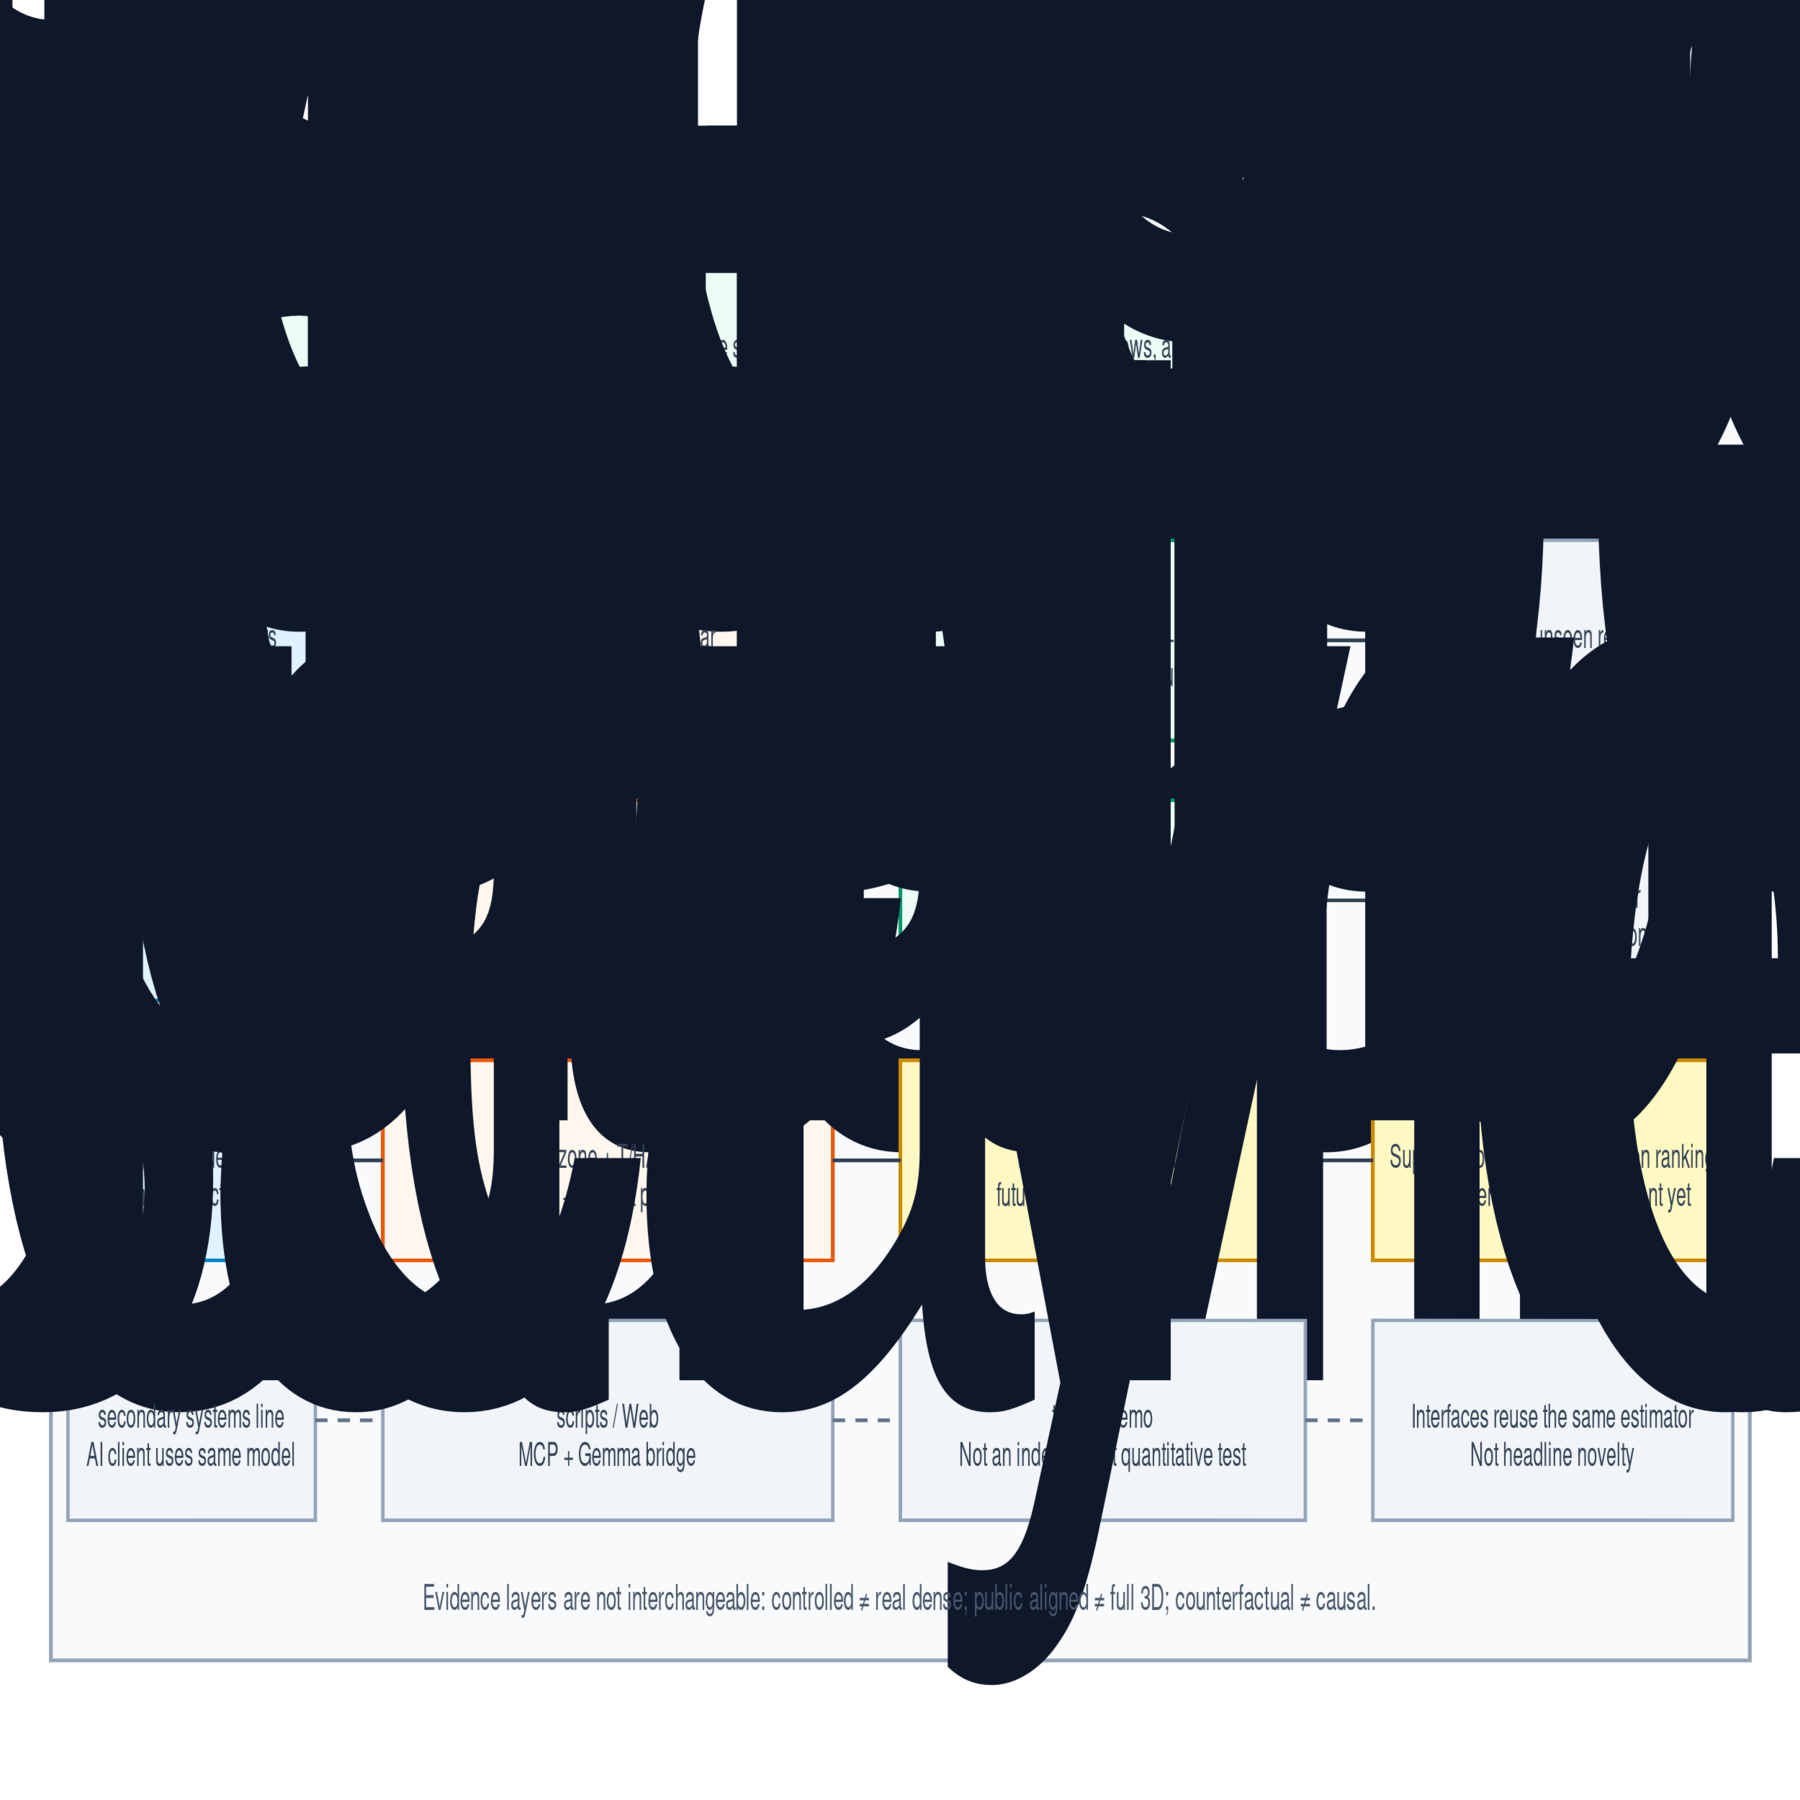
\includegraphics[width=0.96\textwidth]{../thesis/assets/fig_3_1_research_logic_en.png}
\caption{Overall argument map linking the sparse-sensing and non-networked-appliance gap to RQ1--RQ4, method components, the E1--E9 evidence hierarchy, and bounded conclusions. RQ4 is a secondary service line, while E8 remains a future intervention protocol.}
\label{fig:architecture}
\end{figure*}

\section{Related Work}
Digital twins increasingly represent physical systems in manufacturing, infrastructure, and smart buildings \cite{tao2019digitaltwin,fuller2020digitaltwin}. Building reviews emphasize BIM/BMS connectivity, while sparse-sensor spatial estimation remains less explored \cite{cespedes2024bdtreview}. Reduced-order and grey-box models are interpretable alternatives to CFD \cite{bacher2011heatdynamics,hietaharju2018dynamicmodel}; zonal and hybrid models retain dominant non-uniformity at lower cost \cite{teshome2004zonalreview,huljak2025hybrid}. Public BMC telemetry exposes temperatures, fan speeds, and power \cite{bmcdata2026}. Hybrid forecasting can learn simulation--measurement residuals \cite{oh2024hybridmodeling}, and data assimilation shows that finite observations and sensor placement matter \cite{qian2025dafield,chen2007zonalnetwork}. This work couples sparse sensing with appliance-aware influence bases and residual calibration; IDW \cite{shepard1968two} is the geometry-free baseline. Local APIs, a web demo, and an MCP-compatible layer expose the estimator but remain secondary \cite{mcp2025}.

\section{Method}
\subsection{Room, Devices, and Field Model}
The canonical room is a $6.0$ m by $4.0$ m by $3.0$ m rectangular room with eight corner sensing nodes, four on the floor and four on the ceiling. Each node measures temperature, humidity, and illuminance. The room contains three evaluation zones and three appliance classes: an air conditioner, a window, and a light. The web demo represents these appliances as wall or ceiling markers and allows their activations to be toggled.

\begin{figure}[t]
\centering
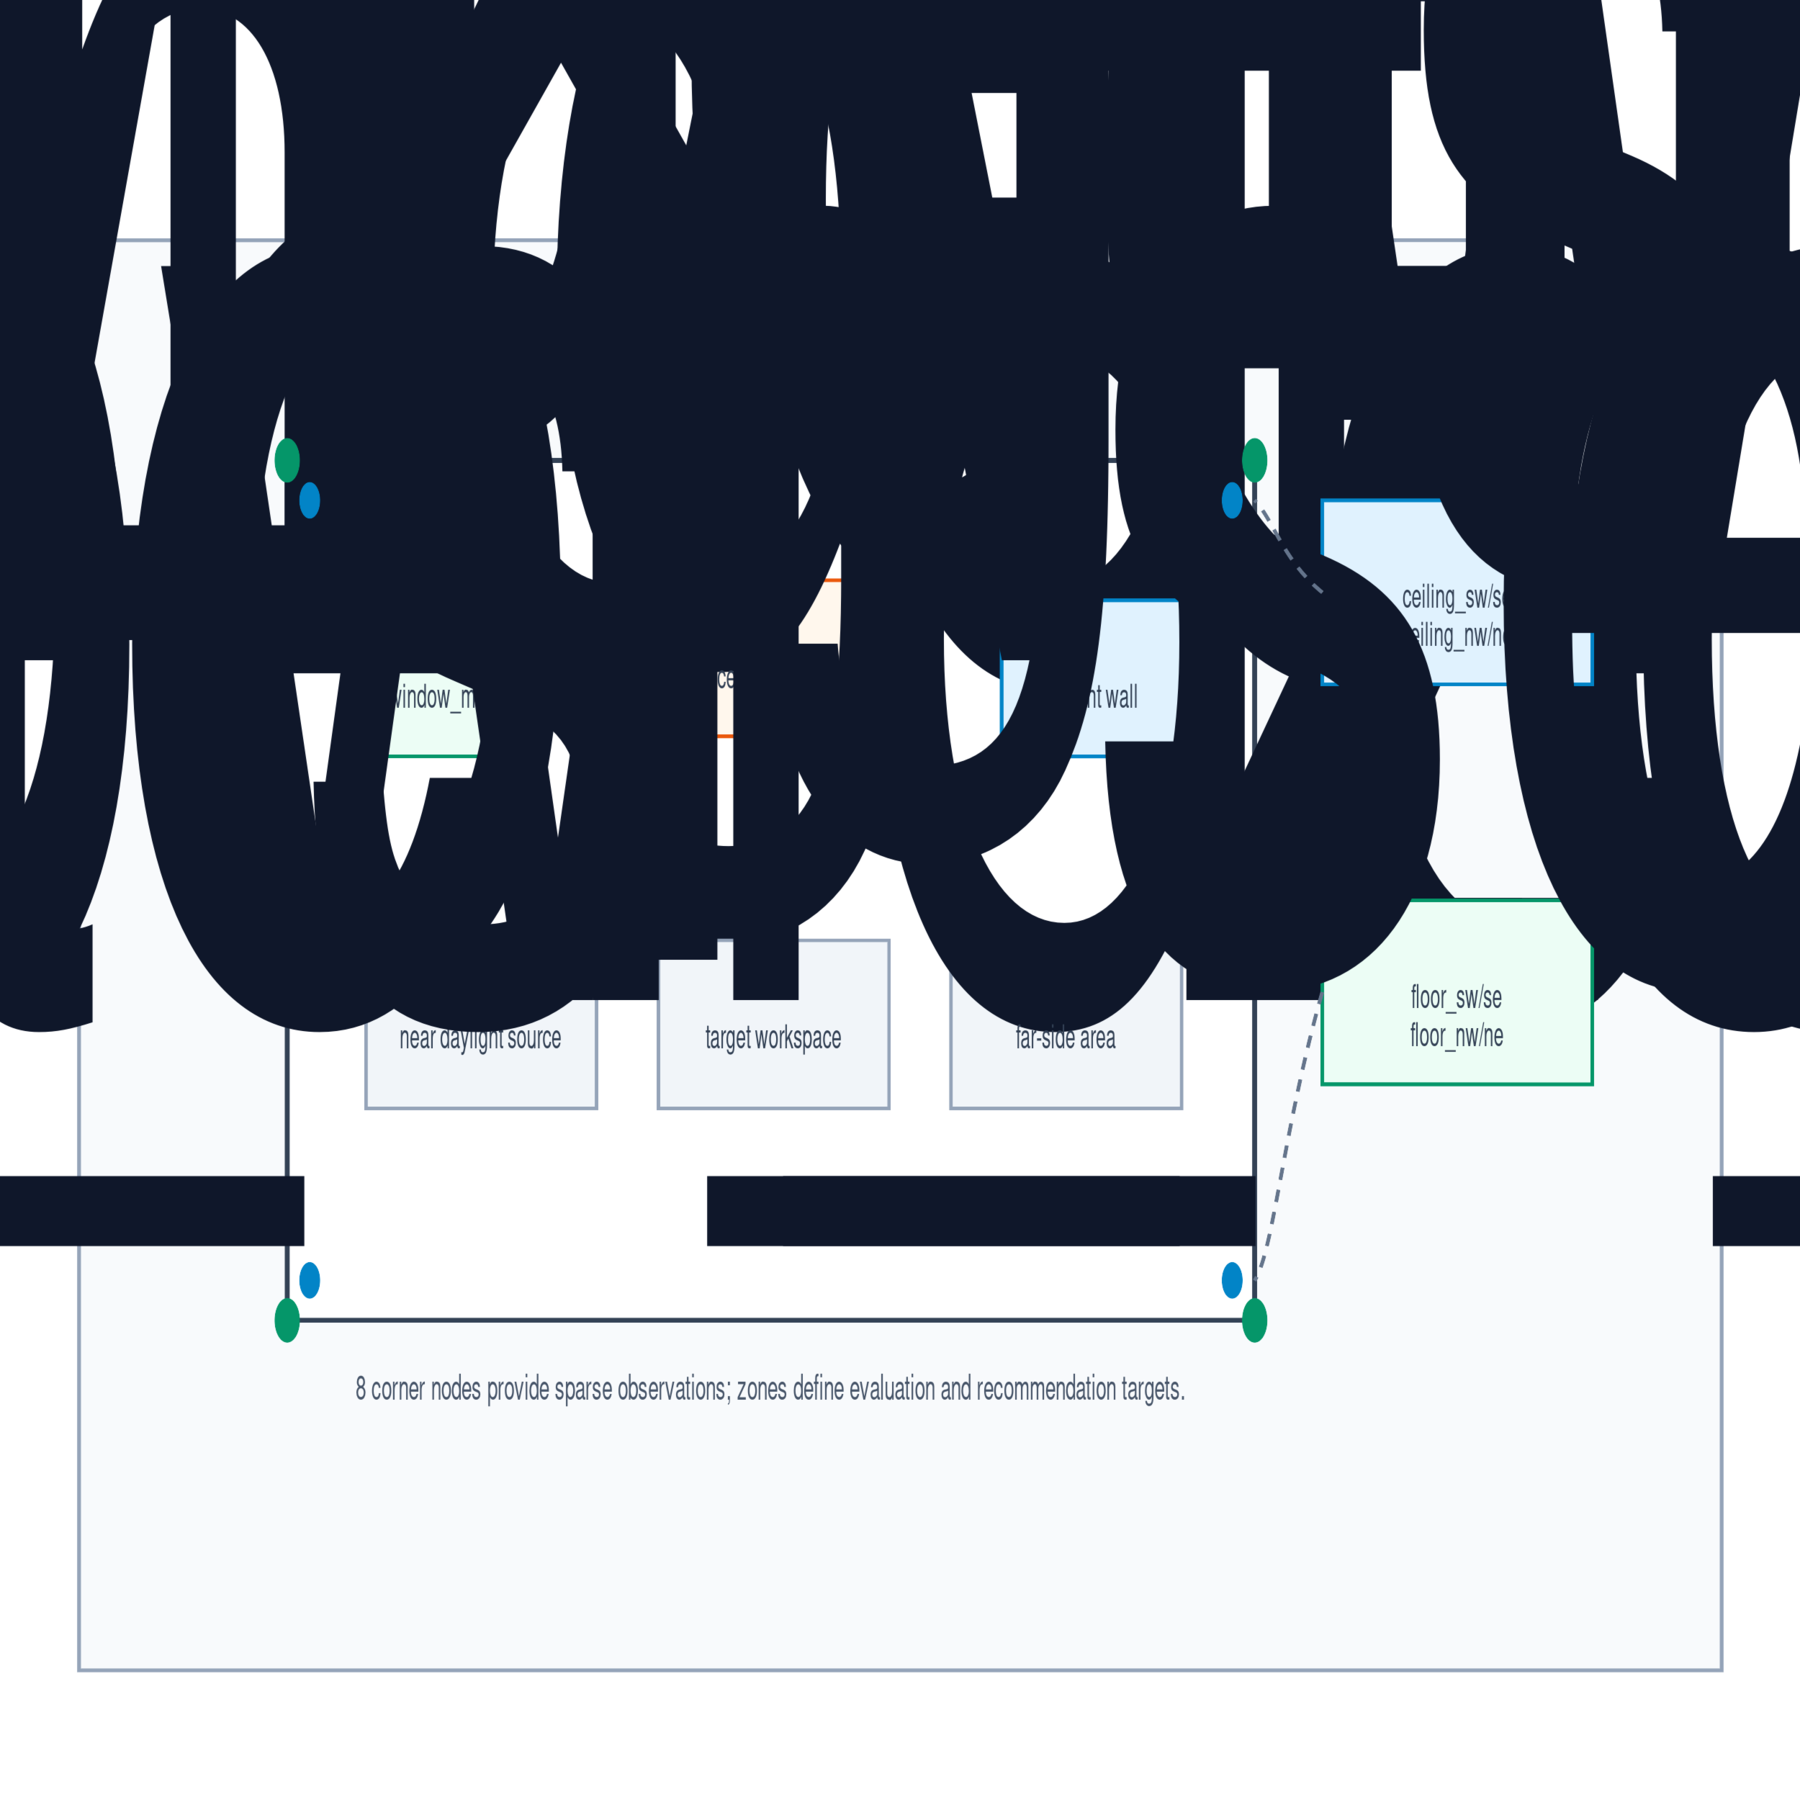
\includegraphics[width=0.96\linewidth]{../thesis/assets/fig_3_3_room_topology.png}
\caption{Room topology, appliance placement, target zones, and the eight floor/ceiling corner sensors.}
\label{fig:room_topology}
\end{figure}

For metric $m\in\{T,H,L\}$ at point $\mathbf{p}=(x,y,z)$ and elapsed time $t$, the estimated field is
\begin{equation}
F_m(\mathbf{p},t)=B_m^{\mathrm{bulk}}(t)+B_m^{\mathrm{local}}(\mathbf{p},t)+\sum_j I_{j,m}(\mathbf{p},t)+C_m(\mathbf{p}).
\end{equation}
The bulk term captures whole-room settling, local terms preserve spatial gradients, $I_{j,m}$ represents appliance influence, and $C_m$ is fitted from sparse sensor residuals. Each appliance influence is modulated by
\begin{equation}
E_j(\mathbf{p},t)=a_j(1-e^{-t/\tau_j})D_j(\mathbf{p})G_j(\mathbf{p}),
\end{equation}
where $a_j$ is activation, $\tau_j$ is a response time constant, $D_j$ is distance attenuation, and $G_j$ is directional gain. The air conditioner lowers temperature and humidity, the window uses outdoor temperature, humidity, and sunlight, and the light primarily raises illuminance with a small heat gain. The lamp direct term uses a cosine beam weight derived from beam angle, an inverse-square distance scale with bounded gain, and line-of-sight obstruction. Window daylight remains an envelope-based daylight term in the reported experiments; an aperture view-factor option is implemented but not used as the default because it increased window-family illuminance error in the current canonical setup.

Direct window and lamp terms underestimate indirect fill light near floors, walls, and furniture. Instead of full ray tracing, illuminance adds a lightweight one-bounce diffuse term
\begin{equation}
I^{\mathrm{refl}}(\mathbf{p},t)=\sum_{s\in\mathcal{S}}\rho_s\bar I_sA_s^{\mathrm{rel}}e^{-\|\mathbf{p}-\mathbf{c}_s\|/\ell_s}\gamma_s(\mathbf{p})V_s(\mathbf{p}),
\end{equation}
where surfaces $\mathcal{S}$ include room boundaries and active furniture faces, $\rho_s$ is reflectance, $\bar I_s$ is direct illuminance at surface center $\mathbf{c}_s$, $A_s^{\mathrm{rel}}$ is normalized area, $\ell_s$ is attenuation length, $\gamma_s$ is diffuse alignment, and $V_s$ is an obstruction term.

\subsection{Sparse Calibration and Learning}
Given predicted sensor value $\hat y_{i,m}$ and observed value $y_{i,m}$, residual $r_{i,m}=y_{i,m}-\hat y_{i,m}$ is used in two steps. First, active-device power scales are fitted by least squares over sensor residuals. Second, a trilinear correction is fitted:
\begin{align}
C_m(x,y,z)={}&c_{0,m}+c_{1,m}X+c_{2,m}Y+c_{3,m}Z+c_{4,m}XY\nonumber\\
&+c_{5,m}XZ+c_{6,m}YZ+c_{7,m}XYZ,
\end{align}
where $X,Y,Z$ are normalized room coordinates. This cannot recover high-frequency turbulence, but it corrects bias, first-order gradients, and corner interactions from the eight observations.
The trilinear form is deliberately matched to the sensing layout. With floor and ceiling sensors at all four horizontal corners, the eight observations constrain the eight coefficients without introducing a high-order surface that would overfit sparse points. The correction should therefore be interpreted as a low-frequency bias and gradient adjustment, not as a substitute for dense flow or lighting measurements. This design keeps the estimator identifiable from the available observations while still letting appliance geometry and dynamics remain in the explicit physical layer.

For non-networked devices, before/after sensor deltas supervise impact learning. The learning event is stored as an appliance-state record rather than as a free-text action label: it includes a record id, device name, applied device state, merged runtime device specifications, indoor baseline, outdoor boundary conditions, furniture state, elapsed time, and before observations. For an air conditioner, the applied state may include activation, mode, setpoint, fan speed or strength, outlet angles, and sweep settings. After observations from the same sensors complete the record. Given metric deltas $\Delta\mathbf{y}_m$ and appliance envelopes in matrix $X$, coefficients are estimated by
\begin{equation}
\boldsymbol{\beta}_m=\arg\min_{\boldsymbol{\beta}}\|\Delta\mathbf{y}_m-X\boldsymbol{\beta}\|_2^2.
\end{equation}
For residual learning, point features include normalized coordinates, elapsed time, indoor/outdoor conditions, base estimates, device activations, calibrated powers, appliance envelopes, and air-conditioner operating state such as mode, setpoint, fan strength, outlet angles, and sweep settings. The hybrid residual layer predicts $R_m(\mathbf{p},t;\theta_m)$ and returns $F_m^{\mathrm{hybrid}}=F_m+R_m$. This is the current-state spatial form used in the reported experiments. Its time-aligned $h$-step generalization is
\begin{equation}
\widehat F_m^{\mathrm{hybrid}}(\mathbf{p},t+h\mid\mathcal{I}_t)
=\widehat F_m^{\mathrm{phys}}(\mathbf{p},t+h\mid\mathcal{I}_t)
\widehat R_m(\mathbf{p},t+h\mid\mathcal{I}_t).
\end{equation}
Here, $h$ is forecast lead rather than a physical coefficient. The physics term carries $t+h$ because it is propagated from information available at forecast origin $t$ to produce the baseline at the same target time as the residual forecast. The information set $\mathcal{I}_t$ may include forecast boundary conditions and planned controls but excludes observations or truth residuals from $t+h$. The present spatial-estimation experiments correspond to $h=0$ and do not constitute a new multi-step forecasting evaluation. Temperature and humidity residual traces can be Fourier low-pass filtered before training because thermal and moisture responses are typically smoothed by heat capacity, air mixing, moisture exchange, and dehumidification. Illuminance uses raw residual labels because lighting, daylight, shadows, occlusion, and reflection can create physically meaningful short-timescale changes that low-pass filtering would remove.

The data flow in Fig.~\ref{fig:data_flow} is intentionally shared between training and runtime use. During learning, raw corner-sensor records, device events, outdoor boundary conditions, and scenario metadata are first time-aligned and normalized, then assembled into the same scenario state used by the service layer. This state is evaluated by the reduced-order estimator to produce base fields and residual labels. The pipeline then branches into least-squares impact learning from before/after sensor deltas and optional hybrid residual training from point-level residual samples, producing learned coefficients, validation summaries, and a checkpoint. At runtime, a user, web interface, or MCP client supplies the current baseline, outdoor conditions, device and furniture states, elapsed or steady-state time, and a query point or target zone. The service rebuilds the scenario state, evaluates the nominal fields, applies sparse correction and the optional residual checkpoint, and returns point or zone estimates. Action ranking is defined only after a decision sample scope is specified, either a single query point or a cluster/zone sample, and after a complete three-factor temperature, humidity, and illuminance target/tolerance vector is supplied. Without those inputs, the service returns estimates only and does not emit recommendations. Given scope and target, each candidate device action is converted into a counterfactual scenario and passed through the same inference path; actions are sorted by predicted comfort-penalty reduction.

\begin{figure}[t]
\centering
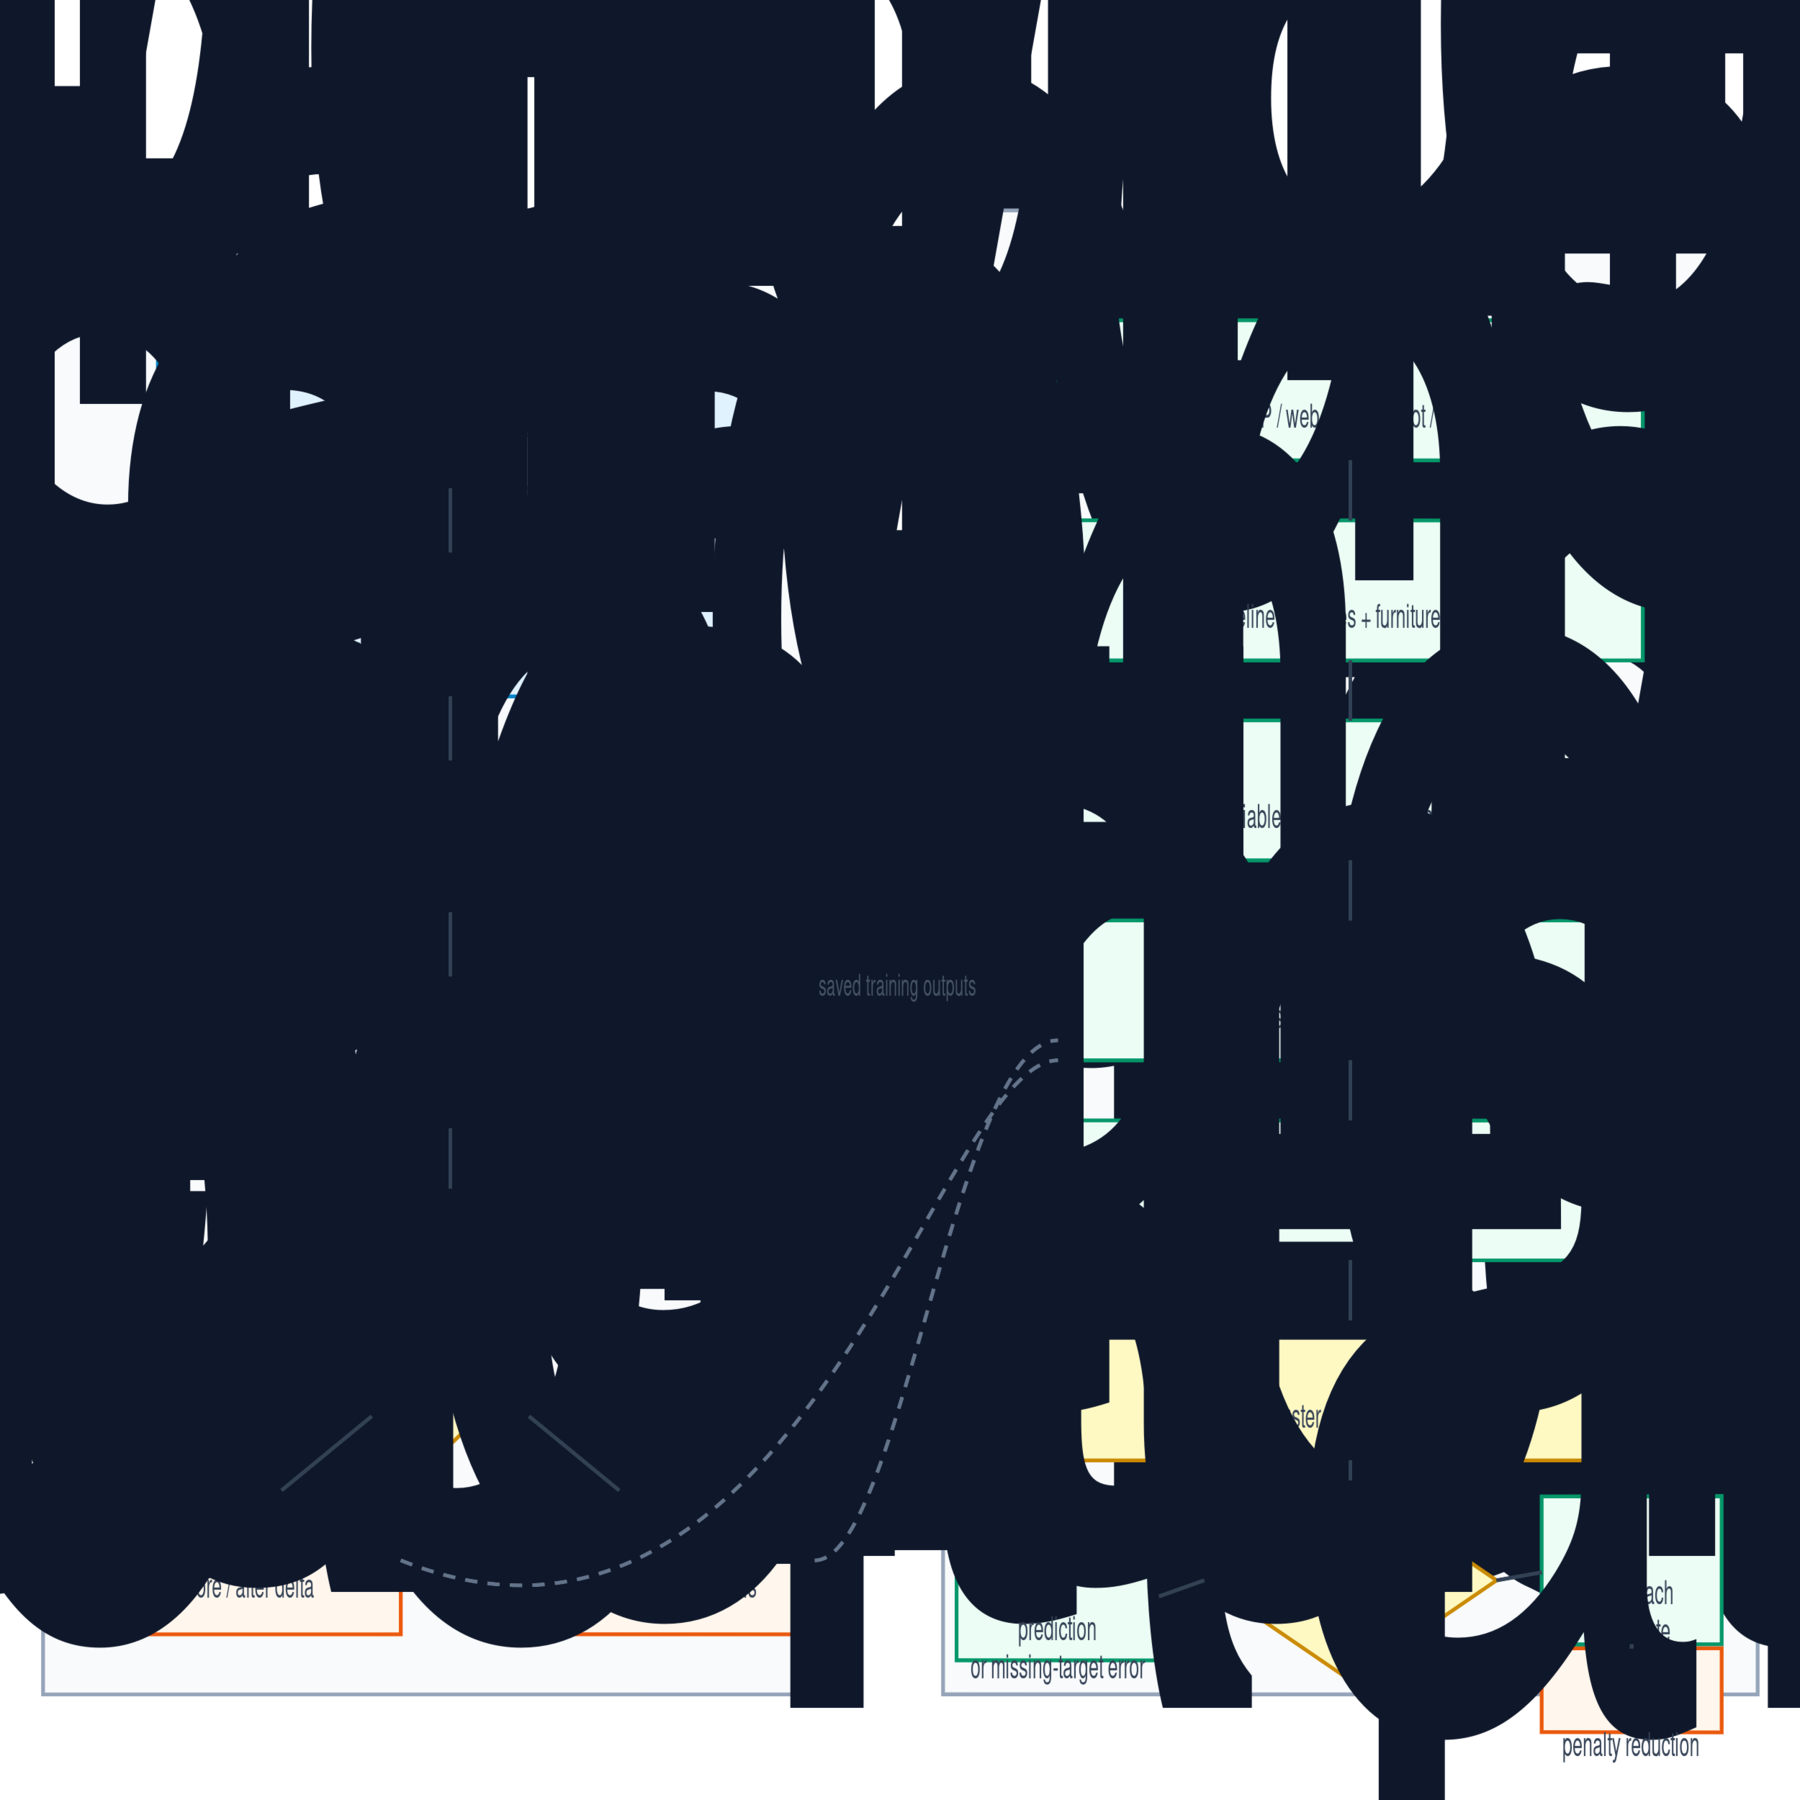
\includegraphics[width=0.99\linewidth]{../thesis/assets/fig_3_5_training_inference_flow.png}
\caption{Shared learning, inference, and recommendation data flow. Learned impact coefficients and the optional residual checkpoint are saved from the training path and reused by the runtime estimator.}
\label{fig:data_flow}
\end{figure}

Candidate control actions are evaluated as model-based counterfactuals. Let $S=\{\mathbf{p}_k\}_{k=1}^{K}$ be the decision sample scope, where $K=1$ is a point query and $K>1$ is a cluster or target-zone sample. For metric $m$, the scope value is $q_m(S)=K^{-1}\sum_k F_m(\mathbf{p}_k,t)$. A weighted comfort penalty is computed from normalized deviations beyond target tolerances for temperature, humidity, and illuminance, and each action is ranked by current penalty minus simulated post-action penalty. AC actions carry a fuller operating state rather than only an on/off flag: cooling, drying, heating, or fan mode; temperature setpoint; fan speed or numeric fan strength; horizontal and vertical outlet angles; and fixed or sweeping airflow. This is recommendation ranking, not closed-loop control; causal validation requires before/after intervention trials.

\section{Implementation and Experimental Setup}
The prototype is implemented as a zero-dependency Python package with modules for entities, scenarios, field simulation, impact learning, hybrid residual training, IDW comparison, action ranking, service APIs, an MCP endpoint, and a rotatable web demo. The shared service layer still supports the reproduction scripts and browser demo, while the MCP endpoint is intentionally narrowed to five runtime tools: environment initialization, elapsed-time or steady-state point sampling, before/after impact-learning records, direct window input, and point-target action ranking from registered devices. The ranking endpoint requires the point coordinates plus a complete temperature, humidity, and illuminance target; missing target fields produce no recommendation. The initialization tool registers the runtime state used by subsequent calls, including the base scenario, indoor baseline, outdoor boundary conditions, device and furniture states, AC mode/setpoint/fan/airflow controls when present, default elapsed or steady-state timing, and the estimator choice.

The service layer is intentionally kept separate from the estimator. A command-line script, the MCP endpoint, and the browser demo call the same scenario and sampling functions, so evaluation results are not produced by a separate code path from the interactive prototype. The browser interface supports metric switching, appliance toggling, AC mode/setpoint/fan-speed/outlet-angle controls, indoor baseline editing, season-weather-time presets, outdoor boundary overrides, point sampling, target-zone summaries, impact-learning output, and estimator switching between the base and hybrid residual fields when a saved checkpoint is available.
This separation also reduces an implementation risk common in demonstration-driven digital twins: the visual interface can change without changing the numerical estimator, and the estimator can be tested from scripts without relying on browser state. The MCP layer is consequently treated as a deployment interface for the same service functions rather than as a separate modeling contribution. In the present paper, this matters because reported MAE values remain tied to reproduction scripts, while MCP point samples, learning records, direct window inputs, and action rankings expose the same runtime estimator without turning validation utilities such as IDW comparison or the full window matrix into MCP-facing claims.

All synthetic full-field experiments use the canonical room and $16\times12\times6$ grid, giving 1152 spatial samples per field. Scenarios are evaluated after an 18-minute settling interval with outdoor temperature $33.0^\circ$C, relative humidity $74.0\%$, and sunlight 32000 lux. The eight canonical scenarios are idle, AC only, window only, light only, AC+window, window+light, AC+light, and all active. Dense synthetic truth is generated by deterministic appliance power adjustments and sensor observations are synthesized from truth sensor predictions with fixed index-based perturbations: temperature adds $0.08((i\bmod4)-1.5)$, humidity adds $0.3((i\bmod4)-1.5)$, and illuminance adds $3.0((i\bmod4)-1.5)$. The main reproduction scripts are \texttt{run\_demo.py}, \texttt{run\_hybrid\_residual\_experiment.py}, \texttt{run\_submission\_readiness\_experiments.py}, \texttt{run\_bedroom\_weekly\_simulation.py}, and \texttt{run\_public\_dataset\_model\_comparison.py}.

The bounded indoor operating and application domain considered in this study is $20$--$30^\circ$C. Outdoor boundary inputs may lie outside that interval, as in the canonical hot-weather case, but they do not extend the claimed range of indoor target states or candidate deployment. Human-comfort ranking therefore uses target tolerances rather than assuming that smaller numerical error proves a need for equally narrow actuation.

Because no single dataset covers room geometry, dense 3-D ground truth, appliance state, and real sparse observations at once, the evaluation uses the layered claim boundary in Table~\ref{tab:claim_scope}. We label the validation items as E1--E9 so that each numerical claim is tied to one evidence layer: E1--E6 are controlled synthetic or robustness experiments, E7 is a real-bedroom sparse-calibration check, E8 is a protocol for future before/after recommendation validation, and E9 is the public task-aligned benchmark. This separation is important because good performance on one layer does not automatically validate the others.

\begin{table}[t]
\caption{Validation Scope and Claim Boundary}
\label{tab:claim_scope}
\centering
\scriptsize
\begin{tabular}{|P{0.23\linewidth}|P{0.24\linewidth}|P{0.23\linewidth}|}
\hline
Evidence item & Supports & Boundary\\
\hline
E1--E4 synthetic full-field, IDW, ablation, and impact-learning checks & 3-D reconstruction, baseline comparison, and component contribution under controlled truth & Simulated room and deterministic perturbations\\
\hline
E5 48-case window matrix & Sensitivity to outdoor temperature, humidity, sunlight, and opening ratio & 34 in-domain cases; 14 out-of-domain stress cases\\
\hline
E6 hybrid residual splits & Residual learnability under default, no-Fourier, and leave-one-scenario-out settings & Scenario-family robustness, not arbitrary-room generalization\\
\hline
E7 seven-day bedroom snapshots & Sparse calibration improves a held-out pillow point & One reference point; no dense real 3-D ground truth\\
\hline
E8 recommendation intervention protocol & Defines measured improvement, success rate, and top-1 regret & Protocol only; not counted as completed validation\\
\hline
E9 SML2010 and CU-BEMS task-aligned benchmarks & External positioning on compatible time-series or zone-level prediction tasks & Not direct validation of the full spatial twin\\
\hline
\end{tabular}
\end{table}

\section{Evaluation}
\subsection{E1--E4 Synthetic Reconstruction and Impact Checks}
Across the eight canonical scenarios, the base estimator achieves average field MAE of 0.0474 for temperature, 0.1765 for humidity, and 2.0269 for illuminance. IDW gives 0.1723, 0.4633, and 54.9052, respectively. Table~\ref{tab:synthetic} summarizes the main comparisons and ablations. Removing appliance-aware feedback produces larger temperature and illuminance errors; removing one-bounce reflection or active-device calibration mainly hurts illuminance. The no-trilinear variant can be lower on dense synthetic humidity and illuminance because trilinear correction enforces sparse sensor consistency rather than guaranteed dense-field monotonic improvement.
This last point is important for interpreting the ablation table. The trilinear correction is fitted from corner observations, so it is optimized for consistency with sparse sensors and for the real-bedroom calibration setting. It is not optimized directly against every dense grid point in the synthetic room. A lower dense-field MAE in the no-trilinear row therefore does not imply that sparse calibration is unnecessary; it indicates that sparse correction and dense synthetic truth are different objectives. For deployment, the estimator must respect measured corner observations first, then use the appliance-aware model to extrapolate the field between them.

\begin{figure}[t]
\centering
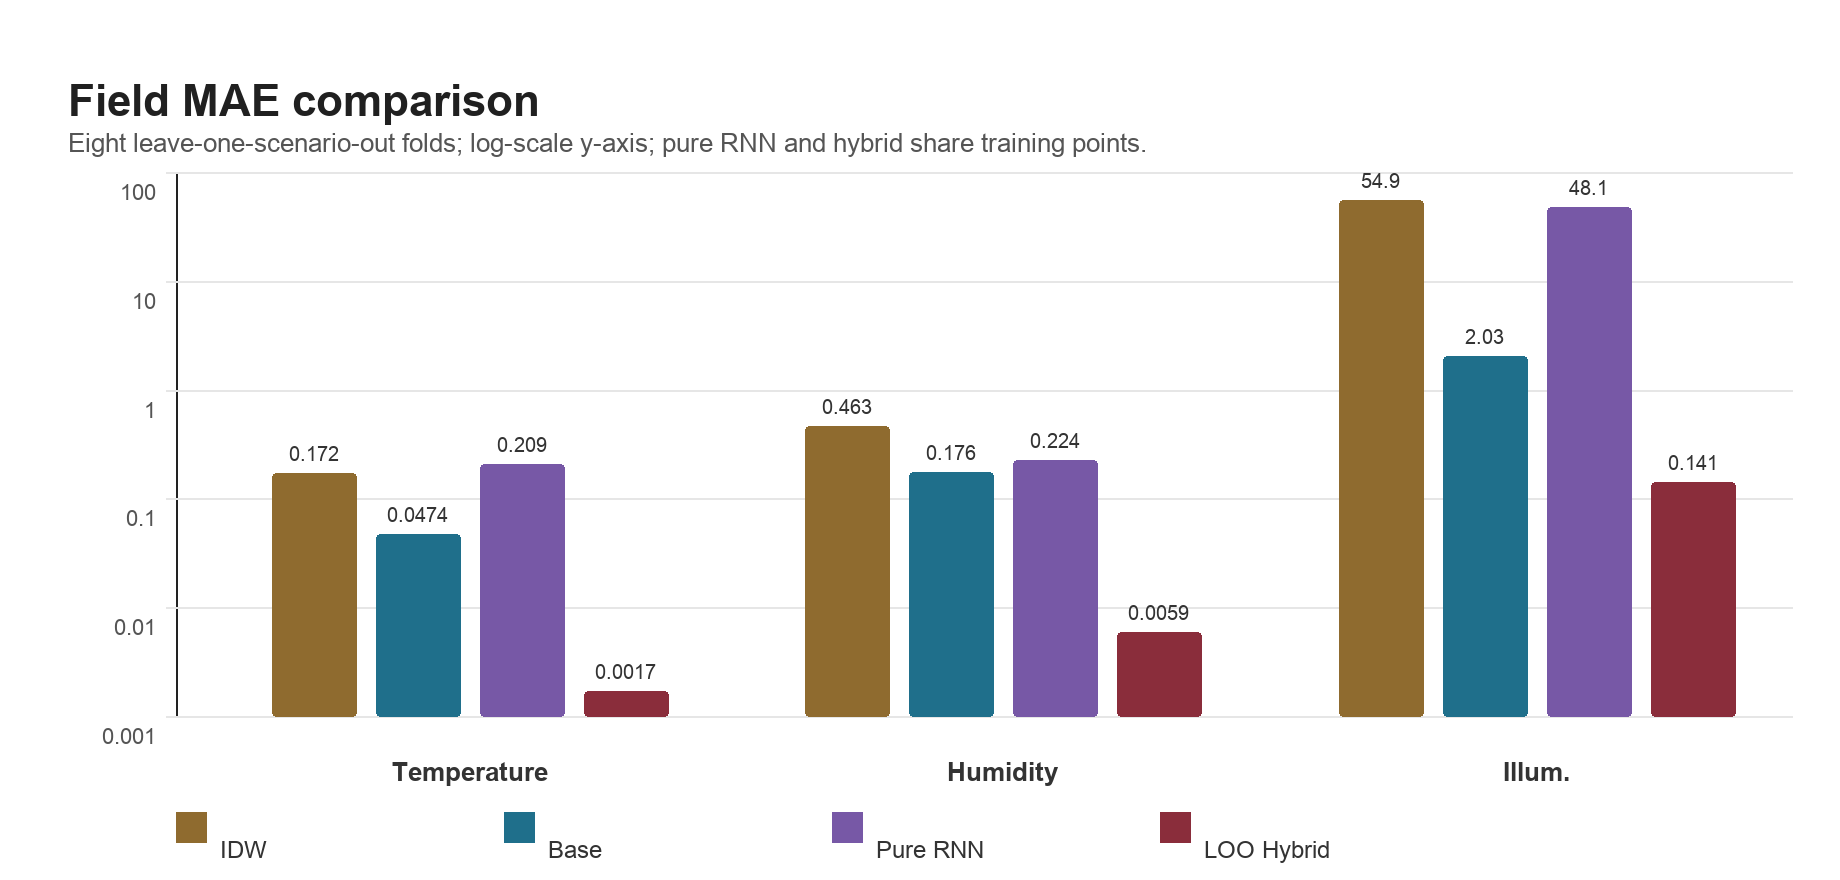
\includegraphics[width=0.96\linewidth]{assets/field_mae_comparison.png}
\caption{Average field MAE for IDW, the base estimator, a pure RNN, and leave-one-scenario-out hybrid residual correction. The y-axis is logarithmic.}
\label{fig:field_mae_comparison}
\end{figure}

\begin{figure}[t]
\centering
\includegraphics[width=0.98\linewidth]{../thesis/assets/fig_5_7_light_only_illum_3d.png}
\caption{Example 3-D illuminance field for the light-only scenario, showing localized lighting influence and reflected fill.}
\label{fig:illum_3d}
\end{figure}

\begin{table}[t]
\caption{Synthetic Field MAE and Robustness Summary}
\label{tab:synthetic}
\centering
\scriptsize
\begin{tabular}{|l|c|c|c|}
\hline
Setting & Temp. & Hum. & Illum.\\
\hline
IDW baseline & 0.1723 & 0.4633 & 54.9052\\
Pure RNN LOO & 0.2091 & 0.2241 & 48.1422\\
Raw nominal & 0.1312 & 0.0842 & 3.5183\\
No reflection & 0.0472 & 0.1762 & 2.4296\\
No calibration & 0.0493 & 0.1772 & 3.3631\\
No trilinear & 0.0446 & 0.0274 & 0.9849\\
Full base & 0.0474 & 0.1765 & 2.0269\\
LOO hybrid avg. & 0.0017 & 0.0059 & 0.1407\\
\hline
\end{tabular}
\end{table}

For impact learning, the AC-only scenario learns negative coefficients for temperature and humidity and near-zero illuminance effect. The light-only scenario learns a strongly positive illuminance coefficient, weak positive heat gain, and near-zero humidity effect. These directions match the intended physical interpretation of the appliances.

\subsection{E6 Pure RNN and Hybrid Residual Correction}
The registered pure Elman RNN reads the same eight sparse observations as ordered spatial tokens and directly predicts absolute field values without physics, IDW, residual, or truth inputs. Each of eight folds trains on 672 points from seven scenarios and tests all 1,152 points of the held-out field. Its average MAE is 0.2091/0.2241/48.1422 and it is lowest in 0/24 fold-factor comparisons; this adverse fixed-architecture result is retained. The default hybrid experiment yields 0.0020/0.0051/0.1370 on its 6/2 split, while the eight-fold LOO hybrid reaches 0.0017/0.0059/0.1407, or 96.41\%/96.66\%/93.06\% reductions from the base estimator. These controlled results do not establish arbitrary-room generalization.

\subsection{E7 Real-Bedroom Snapshot Validation and E8 Intervention Protocol}
We further evaluate calibration on a user-supplied bedroom dataset. The room is a 4.0 m by 4.6 m by 3.2 m bedroom with wall-mounted AC, southeast-facing window, ceiling light, desk lamp, bed, desk, and cabinets. The dataset covers 2026-04-14 to 2026-04-20, with 09:00, 15:00, 22:00, and 02:00 snapshots each day, for 28 cases. Each case provides eight corner observations, appliance activations, outdoor boundary information, and a pillow-location reference observation. Corner sensors are used for active-device calibration and trilinear correction; the pillow point is held out.

Table~\ref{tab:real} shows that calibration reduces pillow-point MAE from 0.8967$^\circ$C, 4.1286\% relative humidity, and 309.0142 lux to 0.1676$^\circ$C, 0.3939\%, and 16.6450 lux. A 20,000-replicate paired date-block bootstrap (seed 20260726) yields mean reductions and 95\% intervals of 0.7291 [0.4582, 1.0232]$^\circ$C, 3.7346 [3.2005, 4.2524]\%RH, and 292.3692 [288.3083, 297.0237] lux; 26/28, 28/28, and 28/28 snapshots improve. Seven overlapping leave-one-date-out folds retain positive minimum reductions of 0.6123$^\circ$C, 3.5551\%RH, and 290.5716 lux. This is an internal sensitivity check over one room, seven dates, and one held-out point, not independent replication or intervention success. Sleep snapshots use a 0 lux illuminance target with 5 lux tolerance so dark sleep conditions are not penalized. These snapshots validate sparse-sensor calibration and point-level estimation, not recommendation efficacy. A versioned E8 trial schema, empty field template, and deterministic analyzer now preregister the before/after endpoints. E8 currently has 0 completed real intervention trials; its summary remains \texttt{NOT\_EVALUATED}, and all efficacy estimates remain null.

\begin{table}[t]
\caption{Real-Bedroom Snapshot Comparison}
\label{tab:real}
\centering
\scriptsize
\begin{tabular}{|l|c|c|c|c|}
\hline
Case & Temp. & Hum. & Illum. & Penalty\\
\hline
Raw pillow MAE & 0.8967 & 4.1286 & 309.0142 & --\\
Calib. pillow MAE & 0.1676 & 0.3939 & 16.6450 & 0.0911\\
Morning calib. & 0.2372 & 0.3695 & 8.6247 & 0.2371\\
Afternoon calib. & 0.1358 & 0.4890 & 11.2235 & 0.0812\\
Night calib. & 0.0913 & 0.2193 & 46.6993 & 0.0459\\
Sleep calib. & 0.2060 & 0.4979 & 0.0326 & 0.0000\\
\hline
\end{tabular}
\end{table}

\subsection{E5 Window Matrix and E9 Public Benchmarks}
The E5 window matrix has 48 time--weather--season cases and retains outdoor conditions as continuous inputs. Within the indoor $20$--$30^\circ$C domain, 34 target-zone results are in range and 14 remain only as stress cases.

SML2010 \cite{romeu2014sml2010} and CU-BEMS \cite{chitalia2020cubems} support only aligned time-series or zone tasks, not matched 3-D truth. Table~\ref{tab:benchmark} retains favorable and adverse cases: persistence remains strong in high-inertia tasks, the registered RNN wins 0/12 cases, and the controlled Kalman/MA comparison splits 6/6 by variable. E11A screens 317 public BMC file-device cases inside 20--30$^\circ$C; only 5 meet the minimum, persistence wins all 5, and thermal balance wins 0.

\begin{table}[t]
\caption{Selected Task-Aligned Benchmark Results}
\label{tab:benchmark}
\centering
\scriptsize
\begin{tabular}{|l|l|c|c|c|}
\hline
Task & Metric & Pers. & LinReg & Proposed\\
\hline
S3 15min temp. & MAE  & 0.233 & 0.093 & \textbf{0.071}\\
S3 15min temp. & Corr. & 0.000 & 0.909 & \textbf{0.950}\\
S3 60min temp. & MAE  & 0.563 & 0.212 & \textbf{0.190}\\
S3 60min illum. & RMSE & 21.93 & 22.76 & \textbf{19.34}\\
S1 15min illum. & MAE  & \textbf{3.42} & 4.02 & 5.35\\
C2 15min illum. & MAE  & \textbf{1.36} & 1.79 & 7.70\\
S2 15min hum. & MAE  & \textbf{0.20} & 0.21 & 0.83\\
\hline
\end{tabular}
\end{table}

\subsection{Validity Considerations}
Dense truth is synthetic; E7 covers one room, seven dates, and one held-out point, while public data validate aligned subtasks only. RNN and injected-noise Kalman results do not generalize to other architectures or deployed sensors. Claims remain within $20$--$30^\circ$C, and action rankings remain counterfactual pending interventions.

\subsection{Bounded AAU Enclosure Transfer}

On 42 mapped AAU locations~\cite{melgaard2026aau,sarikaya2025energy}, E11B (1,641 snapshots) rejects global IDW: nearest-neighbor MAE is 1.175 vs. 1.687~$^\circ$C with 30/42 vs. 6/42 wins (H-ENC-02 unsupported). E11C (1,505 snapshots) lowers MAE from 1.301 to 1.223~$^\circ$C but wins only 21/42 (H-ENC-03 unsupported). E11D role conditioning lowers global-mean MAE/RMSE from 2.3972/2.9748 to 1.6517/2.3648~$^\circ$C, wins 30/42, and gives CI $[0.6867,0.8124]~^\circ$C; H-ENC-04 is predictive, not causal. E11E reaches MAE 1.0187~$^\circ$C but P95 3.7699~$^\circ$C and 25/42 wins; E11G reaches 0.8945/1.5415/3.1013~$^\circ$C but 21/42, so both yield \texttt{no\_candidate\_forwarded}. Two-day E11H commissioning reaches MAE 0.4039~$^\circ$C. Its frozen no-refit E11F map confirms MAE/RMSE/P95 0.3966/0.6723/1.2756~$^\circ$C, 39/42 wins, and CI $[0.5851,0.9274]~^\circ$C. The decision is \texttt{h\_enc\_05\_supported\_within\_campaign}: dates overlap development, while NTC hardware and cross-enclosure validity remain untested.

\section{Discussion and Conclusion}
The appliance-aware model outperforms IDW and the registered pure RNN under controlled truth, while residual calibration improves the sparse real-room point. In a fixed-budget, single-seed SML2010 check, GRU and LSTM are lowest-MAE in 0/12 cases; GRU beats vanilla RNN in 2/12 with median relative MAE reduction $-12.88\%$, and LSTM in 0/12 with $-11.37\%$, so the gated-recurrence hypothesis is unsupported. Public evidence remains task-bounded; dense measurement and interventions are future work, and PID remains unevaluated.

\bibliographystyle{IEEEtran}
\bibliography{references}

\end{document}
